\section{Windkraft}
\begin{minipage}[lt]{10cm}
	max. Windleistung: $P_{max} = \frac{dW}{dt} = \frac{1}{2} \cdot \rho \cdot A \cdot v_1^3$\\
	Leistungsbeiwert: $c_P = \frac{P_W}{P_{max}} = 0.3 \dots \frac{16}{27}$\\
	Windturbinenleistung: $P_W = c_P \cdot P_{max} = c_P \cdot \frac{1}{2} \cdot \rho \cdot A \cdot v_1^3$\\
	Dichte Luft: $\rho_{Luft} \approx 1.29~kg/m^3$
\end{minipage}
\begin{minipage}[rt]{5cm}
	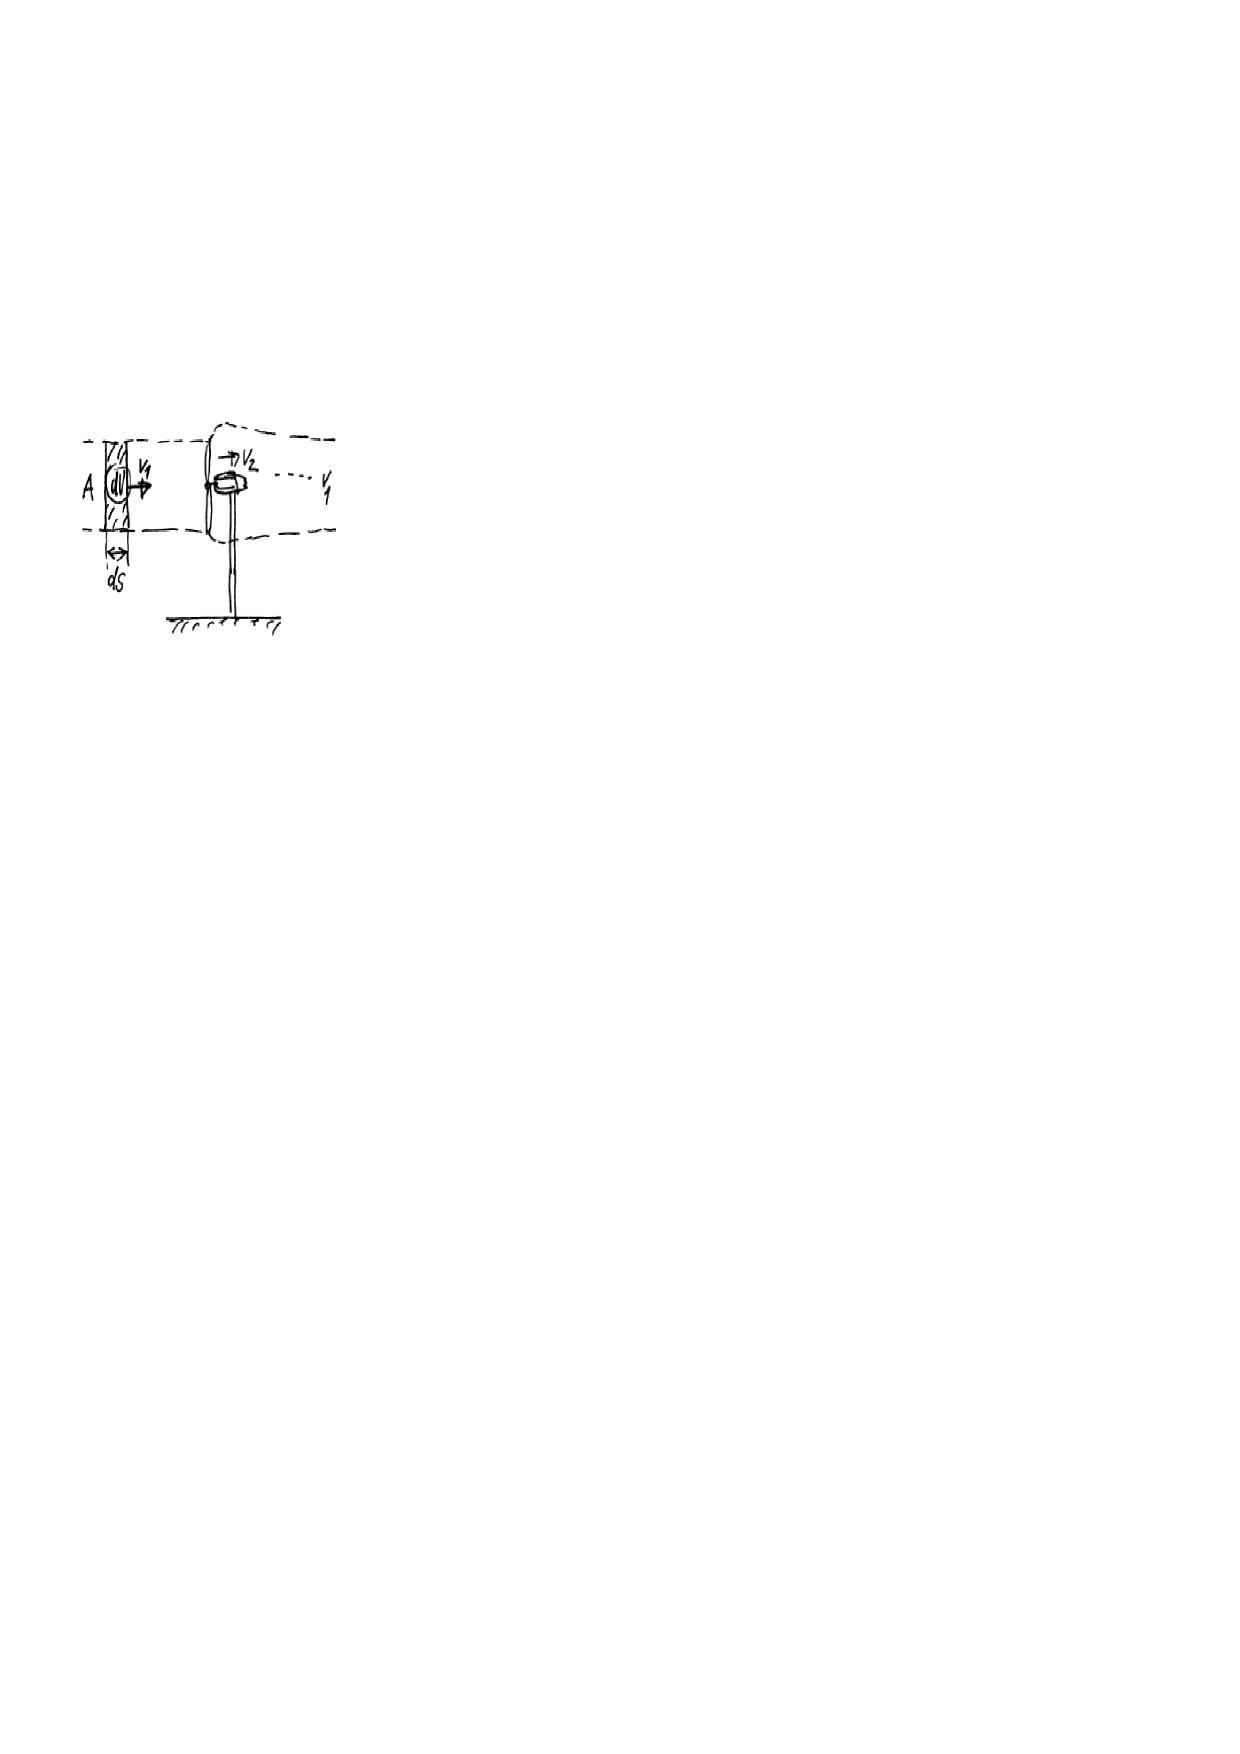
\includegraphics[width=0.7\textwidth]{./images/Wind.pdf}
\end{minipage}
	
		